\documentclass[12pt,a4paper,report]{article}
\usepackage[a4paper, mag=1000, left=2.5cm, right=1cm, top=2cm, bottom=2cm, headsep=0.7cm, footskip=1cm]{geometry}
\usepackage[utf8]{inputenc}
\usepackage[english,russian]{babel}
\usepackage{indentfirst}
\usepackage[dvipsnames]{xcolor}
\usepackage[colorlinks]{hyperref}
\usepackage{listings}
\usepackage{caption}
\usepackage{fancyhdr}
\usepackage{graphicx}
% \usepackage{times}
\DeclareCaptionFont{white}{\color{white}}
\DeclareCaptionFormat{listing}{\colorbox{gray}{\parbox{\textwidth}{#1#2#3}}}
\captionsetup[lstlisting]{format=listing,labelfont=white,textfont=white}
\lstset{% Собственно настройки вида листинга
inputencoding=utf8, extendedchars=\true, keepspaces = true, % поддержка кириллицы и пробелов в комментариях
language=Pascal,            % выбор языка для подсветки (здесь это Pascal)
basicstyle=\small\sffamily, % размер и начертание шрифта для подсветки кода
numbers=left,               % где поставить нумерацию строк (слева\справа)
numberstyle=\tiny,          % размер шрифта для номеров строк
stepnumber=1,               % размер шага между двумя номерами строк
numbersep=5pt,              % как далеко отстоят номера строк от подсвечиваемого кода
backgroundcolor=\color{white}, % цвет фона подсветки - используем \usepackage{color}
showspaces=false,           % показывать или нет пробелы специальными отступами
showstringspaces=false,     % показывать или нет пробелы в строках
showtabs=false,             % показывать или нет табуляцию в строках
frame=single,               % рисовать рамку вокруг кода
tabsize=2,                  % размер табуляции по умолчанию равен 2 пробелам
captionpos=t,               % позиция заголовка вверху [t] или внизу [b]
breaklines=true,            % автоматически переносить строки (да\нет)
breakatwhitespace=false,    % переносить строки только если есть пробел
escapeinside={\%*}{*)}      % если нужно добавить комментарии в коде
}

\begin{document}
  \renewcommand{\chaptername}{}
  \begin{titlepage}
  \begin{center}
    \textbf{МИНИСТЕРСТВО НАУКИ И ВЫСШЕГО ОБРАЗОВАНИЯ РФ}\\[5mm]
    \textsc{
      Федеральное государственное автономное\\
      образовательное учреждение высшего образования\\
      «Национальный исследовательский университет ИТМО»
    }
    \vfill
    \textsc{ФАКУЛЬТЕТ БЕЗОПАСНОСТИ ИНФОРМАЦИОННЫХ ТЕХНОЛОГИЙ}
    \vfill

    \textsc{Организационное и правовое обеспечение информационной безопасности}\\[2mm]
    \textbf{ОТЧЁТ ПО ПРАКТИЧЕСКОЙ РАБОТЕ №3\\[3mm]}
    \end{center}

    \vfill

    \hfill
    \begin{minipage}{.5\textwidth}
    Выполнил:\\[2mm]
    Курятов Евгений Андреевич\\
    группа: N3447\\[2mm]
    
\includegraphics[width=.30\textwidth]{sign}\\[5mm]

    Проверил:\\[2mm]
    Королёва А.А.
    \end{minipage}%
    \vfill
   \begin{center}
    Санкт-Петербург, 2020\ г.
  \end{center}
\end{titlepage}

  \chapter{Результаты работы}
    \section{Перечень документов, подтверждающих введение в организации режима коммерческой тайны:}
    \begin{enumerate}
      \item{приказ об установлении режима коммерческой тайны и утверждении перечня информации, относящейся к коммерческой} тайне;
      \item{положение о коммерческой тайне;}
      \item{положение о порядке работы с документами и информацией, отнесенными к коммерческой тайне;}
      \item{соглашение о неразглашении коммерческой тайны
      \item{журнал доступа к информации, составляющей коммерческую тайну.}
    \end{enumerate}

    \newpage
    \section{Блок-схема порядка увольнения сотрудника по инициативе работодателя.}
    \begin{figure}[h!]
      \begin{center}
        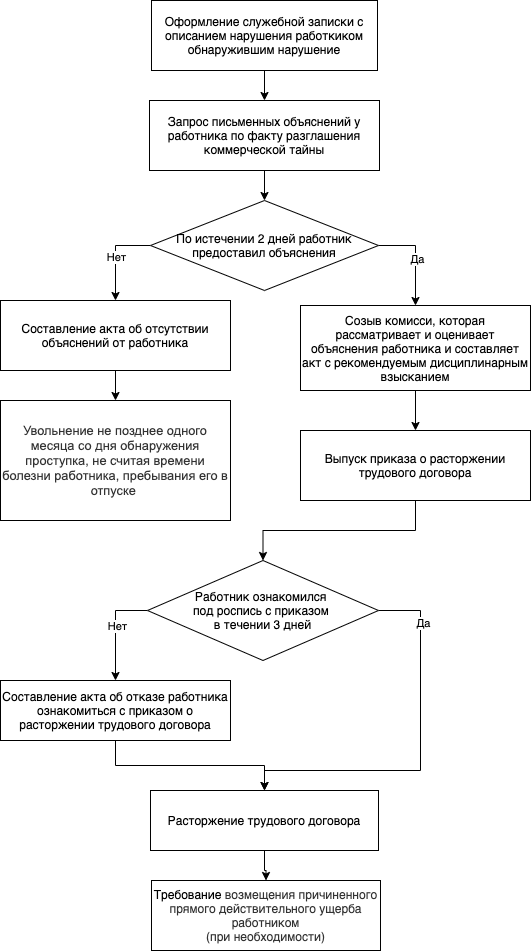
\includegraphics[width=.50\textwidth]{block}
        \caption{Блок-схема порядка увольнения сотрудника по инициативе работодателя.}
      \end{center}
    \end{figure}

    \newpage
    \section{Таблица видов ответственности за разглашение коммерческой тайны.}
    \begin{table}[h!]
    % \centering
      \caption{Виды ответственности за разглашение коммерческой тайны.}
    % \label{tabl:1}
      \begin{tabular}[c]{| l | p{200pt} | p{200pt} |}
      \hline
       & \textbf{Номер статьи, название.} & \textbf{Максимальное наказание} \\
      \hline
      УК РФ &
      Статья 183. Незаконные получение и разглашение сведений, составляющих коммерческую, налоговую или банковскую тайну &	Принудительные работы на срок до пяти лет либо лишением свободы на срок до семи лет.\\
      \hline
      ГК РФ &
      Статья 1472. Ответственность за нарушение исключительного права на секрет производства &
      Возмещение убытков, причиненные нарушением исключительного права на секрет производства, если иная ответственность не предусмотрена законом или договором с этим лицом.\\
      \hline
      ТК РФ &
      Статья 81 п. 6 пп. "в". Расторжение трудового договора по инициативе работодателя &
      Расторжение трудового договора \\
      \hline
      ТК РФ &
      Статья 243 п 7. Случаи полной материальной ответственност &
      Материальная ответственность в полном размере причиненного ущерба \\
      \hline
      КоАП &
      Статья 13.14. Разглашение информации с ограниченным доступом &
      Административный штраф на граждан в размере от пятисот до одной тысячи рублей; на должностных лиц - от четырех тысяч до пяти тысяч рублей. \\

      \hline
      \end{tabular}
    \end{table}

  % \begin{longtable}{||p{76pt}|p{374pt}||}
  %  1-ый Раздел & Текст \\ \hline
  %  2-ой Раздел & Текст \\ \hline
  %  3-ий Раздел & Много текста со списками, который не влезает на страницу. Хочется, чтобы этот текст продолжился на следующей странице \\ \hline
  %  4-ый Раздел & Текст \\
  %  \end{longtable}

\end{document}
